% Copyright (C) 2012 Shi.Zhan <g.shizhan.g@gmail.com>
%
% Permission is hereby granted, free of charge, to any person obtaining a copy of this software and associated documentation files (the "Software"), to deal in the Software without restriction, including without limitation the rights to use, copy, modify, merge, publish, distribute, sublicense, and/or sell copies of the Software, and to permit persons to whom the Software is furnished to do so, subject to the following conditions:
%
% The above copyright notice and this permission notice shall be included in all copies or substantial portions of the Software.
%
% THE SOFTWARE IS PROVIDED "AS IS", WITHOUT WARRANTY OF ANY KIND, EXPRESS OR IMPLIED, INCLUDING BUT NOT LIMITED TO THE WARRANTIES OF MERCHANTABILITY, FITNESS FOR A PARTICULAR PURPOSE AND NONINFRINGEMENT. IN NO EVENT SHALL THE AUTHORS OR COPYRIGHT HOLDERS BE LIABLE FOR ANY CLAIM, DAMAGES OR OTHER LIABILITY, WHETHER IN AN ACTION OF CONTRACT, TORT OR OTHERWISE, ARISING FROM, OUT OF OR IN CONNECTION WITH THE SOFTWARE OR THE USE OR OTHER DEALINGS IN THE SOFTWARE.
%
% 课程:人机交互技术及应用
% 班级:传播学1001班
% 课时:40学时,2012年秋季1~10周,每周一、三
% 地点:东九楼D212
% 主页:http://code.google.com/p/hci-course/
% 教师:施展 
% 单位:华中科技大学 武汉光电国家实验室
%
\documentclass{beamer}
\usepackage{fontspec,xunicode,xltxtra,beamerthemesplit}
%\usetheme{Hannover} % White background
\usetheme{Berkeley} % Blue background
\setsansfont[Mapping=tex-text, ItalicFont={Courier Italic}]{Microsoft YaHei}

% 中文环境自动换行
\XeTeXlinebreaklocale "zh"
\XeTeXlinebreakskip = 0pt plus 1pt

% 中文环境修正导航栏
\makeatletter
\def\beamer@linkspace#1{
	\begin{pgfpicture}{0pt}{-1.5pt}{#1}{5.5pt}
		\pgfsetfillopacity{0}
		\pgftext[x=0pt,y=-1.5pt]{.}
		\pgftext[x=#1,y=5.5pt]{.}
	\end{pgfpicture}
}
\makeatother

% diagrams
\usepackage{tikz}
\usetikzlibrary{arrows,positioning} 
\tikzset{
    %Define standard arrow tip
    >=stealth',
    %Define style for boxes
    punkt/.style={
		rectangle,
		rounded corners,
		draw=black, very thick,
		text width=6.5em,
		minimum height=2em,
		text centered},
	line/.style = {
		->,
		draw,
		text centered,
		-latex'}
}

\title{人机交互技术}
\author{施展}
\institute{华中科技大学~武汉光电国家实验室}
\date{\today}
\titlegraphic{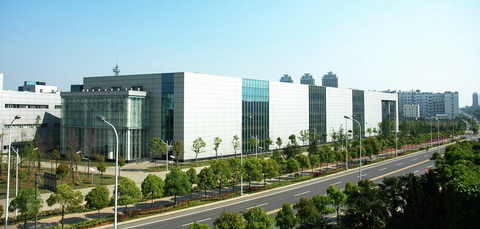
\includegraphics[width=3.5cm]{images/wnlo.jpg}}

\begin{document}

\begin{frame}
	\titlepage
\end{frame}

\begin{frame}
	\frametitle{内容提要}
	\tableofcontents
\end{frame}

\section{第五讲}
\begin{frame}
	\frametitle{第五讲 界面设计}
	\begin{itemize}
		\item 掌握图形用户界面的主要思想和设计的一般原则。
		\item 了解用户、用户体验、用户交互分析以及设计流程。
		\item 掌握任务分析方法方法,重点掌握:
		\begin{itemize}
			\item 使用行为分析、顺序分析、协作关系分析。
		\end{itemize}
		\item 掌握以用户为中心的界面设计方法。
	\end{itemize}
\end{frame}

\subsection{界面设计原则}
\begin{frame}
	\frametitle{界面设计原则}
	\begin{itemize}
		\item 根据表现形式,用户界面分为
		\begin{itemize}
			\item 命令行界面
			\item 图形界面
			\item 多通道用户界面
		\end{itemize}
	\end{itemize}
\end{frame}

\begin{frame}
	\frametitle{图形用户界面的主要思想}
	\begin{itemize}
		\item 图形用户界面的三个重要思想
		\begin{itemize}
			\item 桌面隐喻\\\textit{desktop metaphor}
			\item 所见即所得\\\textit{What You See Is What You Get, WYSIWYG}
			\item 直接操纵\\\textit{Direct manipulation}
		\end{itemize}
	\end{itemize}
\end{frame}

\begin{frame}
	\frametitle{桌面隐喻}

\end{frame}

\begin{frame}
	\frametitle{所见即所得}

\end{frame}

\begin{frame}
	\frametitle{直接操纵}

\end{frame}

\begin{frame}
	\frametitle{图形用户界面~{\small 一般性原则}}

\end{frame}

\subsection{理解用户}
\begin{frame}
	\frametitle{理解用户}

\end{frame}

\begin{frame}
	\frametitle{所谓``用户''}

\end{frame}

\begin{frame}
	\frametitle{用户体验}

\end{frame}

\begin{frame}
	\frametitle{用户的区别}

\end{frame}

\begin{frame}
	\frametitle{用户交互分析}

\end{frame}

\subsection{设计流程}
\begin{frame}
	\frametitle{设计流程}
	\begin{tikzpicture}[node distance=0.5cm, auto,]
		\node[punkt] (a) {用户的观察和分析};
		\node[punkt, right=of a] (b) {设计};
		\node[punkt, right=of b] (c) {实施};
		\path[line]	(a)--(b);
		\path[line]	(b)--(c);
	\end{tikzpicture}
\end{frame}

\begin{frame}
	\frametitle{用户的观察和分析}
	\begin{itemize}
		\item 情境访谈 Contextual Interviews\\{\tiny 走进用户的现实环境,尽量了解你的用户的工作方式、生活环境等情况。}
		\item 焦点小组 Focus Groups\\{\tiny 组织一组用户进行讨论,让你更了解用户的理解、想法、态度和需求。}
		\item 单独访谈 Individual Interviews\\{\tiny 一对一的用户讨论,让你了解某个用户是如何工作,使你知道用户的感受、想要什么及其经历等。}
	\end{itemize}
\end{frame}

\begin{frame}
	\frametitle{设计}
	\begin{itemize}
		\item 对象模型化: \\{\tiny 将用户分析的结果按照讨论的对象进行分类整理,并且以各种图示的方法描述其属性、行为和关系。}
		\item 低真视图 Low-fidelity Prototype\\{\tiny 比较抽象的视图有利于进行逻辑分析。}
		\item 高真视图 High-fidelity Prototype\\{\tiny 比较具体的视图更接近于人机界面的最终表达。}
	\end{itemize}
\end{frame}

\begin{frame}
	\frametitle{实施}
	\begin{itemize}
		\item 设计师对高真设计原型进行最后的调整,并且撰写产品的设计风格标准(Style Guide),产品各个部分风格的一致性由该标准保证。
		\item 产品实施或投入市场后,面向用户的设计并没有结束,而是要进一步的搜集用户的评价和建议,以利于下一代产品的开发和研制。
	\end{itemize}
\end{frame}

\subsection{任务分析}
\begin{frame}
	\frametitle{任务分析}

\end{frame}

\subsection{以用户为中心的界面设计}
\begin{frame}
	\frametitle{以用户为中心的界面设计}

\end{frame}

\section{小结}
\begin{frame}
	\frametitle{小结}
	\begin{itemize}
		\item 理解人机界面设计的一般原则
		\item 掌握以用户为中心的界面设计方法
	\end{itemize}
\end{frame}

\begin{frame}
	\frametitle{参考文献}
	\bibliographystyle{plain}
	\bibliography{hci}
\end{frame}

\end{document}